\section{Compactness} 

  Now we move onto another pillar of topology: compactness. I personally think compactness is the hardest conceptually, so I will provide a lot of explanation on it here. The thing to keep in mind when talking about compactness is that it describes a space being finite or not being able to escape to infinity.  

  \begin{definition}[Covers]
    A collection $\C$ of subsets of a space $X$ is said to \textbf{cover} $X$, or to be a \textbf{covering} of $X$, if the union of the elements of $\C$ is equal to $X$. It is called an \textbf{open covering} of $X$ if its elements are open subsets of $X$. 
  \end{definition}

\subsection{Open Cover Compactness}
  
  \begin{definition}[Compact Space]
    A topological space $X$ is said to be \textbf{compact} if every open covering of $X$ contains a finite subcovering (i.e. a finite collection of subcovers) of $X$. If $K \subset X$ is a compact topological space in the subspace topology, then $K$ is said to be a \textbf{compact subspace} of $X$. 
  \end{definition}

  Note that compactness is a property of a topological space in its entirety. This is opposed to considering open and closed sets, which exist as a subset of a topological space. While openness behaves differently depending on its embedding space, compactness stays constant. Therefore, we don't have to worry about talking about which space a compact set is embedded in. However, we will provide a definition for which it makes sense to talk about compact \textit{subsets} of a space. 

  \begin{definition}[Compact Subspaces]
    Given topological space $X$ and $A \subset Y$, we call $A$ a \textbf{compact subspace} of $X$ if either of the two equivalent conditions are met. 
    \begin{enumerate}
      \item $A$ is a compact space with respect to the subspace topology endowed from $X$. 
      \item If every $X$-open cover of $A$ has a finite subcover of $A$. 
    \end{enumerate}
  \end{definition}
  \begin{proof}
    We can prove bidirectionally. 
    \begin{enumerate}
      \item Suppose that $K$ is compact in $X$. Then given any open cover $\{U_\alpha\}_\alpha$ of $K$, there exists a finite subcover $\{U_i\}_{i}$. Now let there exist an open cover $\{V_\alpha\}$ in $Y$, but every $V_\alpha = U_\alpha \cap Y$ for some $U_\alpha$ open in $X$. Therefore, we can take the finite subcover $\{V_i = V_i \cap Y\}_i$. 

      \item Suppose that $K$ is compact in $Y$. Then given any open cover $\{V_\alpha\}$ of $K$, there exists a finite subcover $\{V_i\}_i$. Now let there exist an open cover $\{U_\alpha\}$ in $X$. Then we set $\{V_\alpha = U_\alpha \cap Y\}_\alpha$, which has a finite subcover $\{V_i = U_i \cap Y\}$, and therefore we can take $\{U_i\}$ as our finite subcover in $X$. 
    \end{enumerate}
  \end{proof}
   
  The concept of compactness does not seem intuitive at first glance. The reason why compactness is such an important property for a space to have is because $X$ being compact tells us that we can \textit{always} analyze the entire $X$ using a finite union of open sets, which can simplify the space greatly. That is, it a measure of finiteness of a space. You should realize that it is much easier to prove that a space is \textit{not} compact, since all we have to do is find a \textit{single} covering that doesn't contain a finite subcovering. 

  \begin{example}[Non-Compact Spaces]
    We show some examples of non-compact spaces. 
    \begin{enumerate}
      \item $\mathbb{R}$ is not compact since given the open covering $\mathcal{F} = \{ (x, x + 1) \subset \mathbb{R} \mid x \in \mathbb{R} \}$, then if we assume that $\mathcal{F}$ has a finite subcovering, it is the case that $\max\{x_1, x _2, \ldots, x_n \} + 1 \not\in \mathcal{F}$, so this is not a covering. 
      \item For $\mathbb{R}$, you can also get a nested covering $\{(-r, +r) \mid r > 0\}$, which also has no finite subcovering. 

      \item Take $X = (1, 1)$ and take $\mathcal{F} = \{ (\frac{1}{n}, 1] \mid n \in \mathbb{N} \}$, which is a cover but has no finite subcover. 
    \end{enumerate}
  \end{example}

  \begin{example}[Open Square is Not Compact]
    The subset $Y \coloneqq (0,1) \times (0,1) \subset \mathbb{R}^2$ is not compact. That is, we can choose to cover the subspace by the finite union of open sets. 
    \begin{equation}
      [0,1]^2 \subset \bigcup_{k=0}^\infty \Big( \frac{2^k - 1}{2^k}, \frac{2^{k+1} - 1}{2^{k+1}} \Big) \times (0,1)
    \end{equation}

    \begin{figure}[H]
      \centering 
      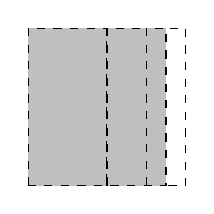
\begin{tikzpicture}[scale=2]
        \draw[dashed] (0,0) rectangle (1,1);
        \draw[dashed, fill=lightgray] (0,0) rectangle (0.5,1);
        \draw[dashed, fill=lightgray] (0.5,0) rectangle (0.75,1);
        \draw[dashed, fill=lightgray] (0.75,0) rectangle (0.875,1);
      \end{tikzpicture}
      \caption{We show the first three elements of the infinite union that covers the open square. }
      \label{fig:closed_square_compact}
    \end{figure}
  \end{example}

  \begin{example}[Finite Sets are Always Compact]
    A finite set $S$ is compact with respect to any topology, because there are only a finite number of open sets to begin with, so every open cover is a finite cover. 
  \end{example}

  According to Terry Tao, a compact set is ``small,'' in the sense that it is easy to deal with. While this may sound counterintuitive at first, since $[0,1]$ is considered compact while $(0,1)$, a subset of $[0,1]$, is considered noncompact. More generally, a set that is compact may be large in area and complicated, but the fact that it is compact means we can interact with it in a finite way using open sets, the building blocks of topology. That finite collection of open sets makes it possible to account for all the points in a set in a finite way. This is easily noticed, since functions defined over compact sets have more controlled behavior than those defined over noncompact sets. Similarly, classifying noncompact spaces are more difficult and less satisfying. 

  In general, it's pretty easy to prove that a set is not compact. We just need to find one example of an open cover that does not have a finite subcover. To prove that set \textit{is} compact, we must show that for \textit{every} open cover, we can get a finite subcover. 

  \begin{theorem}[Closed Subsets of Compact Sets are Compact]
    Every closed subset of a compact space is compact. 
  \end{theorem}
  \begin{proof}
    This proof is quite trivial. Let $Y$ be a closed subset of compact space $X$. Given a covering $\mathcal{C}$ of $Y$ by sets open in $X$, let us form an open covering $\B$ of $X$ by adjoining to $\mathcal{C}$ the single open set $X \setminus Y$. Then, we an see that both $\B$ and $\mathcal{C} \cup (X \setminus Y)$ covers $X$. 
    \begin{equation}
      \B = \mathcal{C} \cup (X \setminus Y)
    \end{equation}
    Since $\B$ is finite, the right hand side must also be expressible as a finite union. Looking through $\B$, we can throw away all the open sets that are entirely in $X \setminus Y$. What remains is a finite covering of $Y$. 
  \end{proof}

  The converse is not necessarily true, unless we have Hausdorff spaces. 

  \begin{theorem}[Compact Subsets of Hausdorff Spaces are Closed]
    If $X$ is Hausdorff and $A \subset X$ is compact. Then $A$ is closed in $X$. 
  \end{theorem}
  \begin{proof}
    We wish to show that $X \setminus A$ is open. Let $x \in X \setminus A$. Then, for each point $a \in A$, we can choose disjoint neighborhoods $U_a \ni x$ and $V_a \ni a$ (using the Hausdorff condition). The collection 
    \begin{equation}
      \{V_a \mid a \in A\}
    \end{equation}
    is an open covering of $A$. Since $A$ is compact, there must exist a finite subcover $V_1, V_2, \ldots , V_n$. Therefore, $\cup_{i=1}^{n} V_i$ contains $Y$ and is disjoint from the intersection of open neighborhoods of $x$
    \begin{equation}
      U \coloneqq \bigcap_{i=1}^n U_i
    \end{equation}
    Therefore, $U$ is an open neighborhood of $x_0$, disjoint from $A \implies X \setminus A$ is open $\implies A$ is closed.
  \end{proof}

  But is it minimal? It turns out that if we don't have Hausdorff, then a compact subset is not necessarily closed. 

  \begin{example}[Line with 2 Origins]
    Consider the line with 2 origins, $L = (-\infty, 0) \cup (0, +\infty) \cup \{r, s\}$. Then $A = \{r\} \cup (0, 1] = [0, 1]$ is not compact, but it is not closed since $r$ is also a limit point. 
  \end{example}

  \begin{lemma}[Compact Subsets and Points Can Be Separated in Hausdorff Space]
    If $Y$ is a compact subset of a Hausdorff space $X$ and $x$ is not in $Y$, then there exist disjoint open sets $U$ and $V$ of $X$ containing $x$ and $Y$, respectively. 

    \begin{figure}[H]
      \centering 
      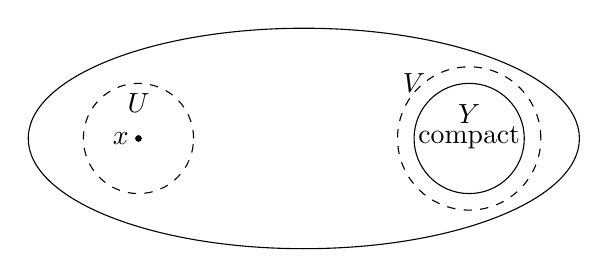
\begin{tikzpicture}[scale=0.7]
        \draw (0,0) ellipse (5 and 2);
        \draw[dashed] (-3,0) circle (1);
        \draw[fill] (-3,0) circle (0.05);
        \node[left] at (-3,0) {$x$};
        \draw (3,0) circle (1); 
        \node[below] at (3,0.8){$Y$};
        \node[below] at (3, 0.4){compact};
        \node[above] at (-3,0.3) {$U$};
        \draw[dashed] (3,0) circle (1.3); 
        \node at (2,1) {$V$};
      \end{tikzpicture}
      \label{fig:hausdorff_compact}
    \end{figure}
  \end{lemma}

  \begin{theorem}[Continuous Mappings from Compact to Hausdorff Spaces]
    Let $X$ be compact, $Y$ Hausdorff, and $f: X \to Y$ be a continuous map. Then, $f$ is a closed map, and moreover, 
    \begin{enumerate}
      \item $f$ injective $\implies$ $f$ is an embedding. 
      \item $f$ surjective $\implies$ $f$ is a quotient map. 
      \item $f$ bijective $\implies$ $f$ is a homeomorphism. 
    \end{enumerate}
  \end{theorem}
  \begin{proof} 
    We prove the four statements. 
    \begin{enumerate}
      \item To see that $f$ is a closed map, let $C \subset X$ be closed. Then $C$ is compact, and so $f(C)$ is also compact. But since $Y$ is Hausdorff, $f(C)$ is closed. 
      \item 
    \end{enumerate}
  \end{proof}

  The previous theorem is nice in that we can prove a lot of the nice properties of topological spaces without doing much work. Note that compactness and Hausdorff goes very well together in that you can get a lot more out of a space when they are together. 

  \begin{definition}[Isolated Point]
    A point $x$ is called an \textbf{isolated point} if $\{x\}$ is an open set. 
  \end{definition}

  \begin{theorem}[Uncountability of Compact Hausdorff Spaces]
    If $X$ is a nonempty, compact, Hausdorff space with no isolated points, then $X$ is uncountable. 
  \end{theorem}
  \begin{proof}
    
  \end{proof}

  Thus, any closed interval in $\mathbb{R}$ is uncountable. We didn't need to use decimal expansions to prove it. 

  \begin{corollary}
    If $F$ is closed and $K$ is compact, then $F \cap K$ is compact. 
  \end{corollary}

  Now lets prove something more set-theoretic about compact sets, namely its cardinality. 

  \begin{theorem}[Nested Sequence Theorem]
    If $X$ is compact, then for any sequence of closed, nonempty sets $C_1 \supset C_2 \supset \ldots$, we must have 
    \begin{equation}
      \bigcup_{n=0}^{\infty} C_n \neq \emptyset
    \end{equation}
  \end{theorem}

  Now we present another theorem in analysis that is actually a topological property. 

  \begin{theorem}[Extreme Value Theorem][thm:evt]
    Let $X$ be compact and $f: X \rightarrow \mathbb{R}$ be continuous. Then $f$ attains both its maximum and minimum in $X$.  
  \end{theorem}
  \begin{proof}
    $f$ continuous must imply that $f(X)$ is compact in $\mathbb{R}$, which means that it is closed and bounded. Since it is bounded, it must have a least upper bound. Since it's closed, it must contain its least upper bound, and so attains its maximum. Similarly for minimum.
  \end{proof}

  The theorem says that $f: [a, b] \to \mathbb{R}$ is bounded, and that bound is \textit{realized} by something. Note that for function on noncompact $(-1, 1)$---say $f(x) = x$---it is bounded but the extrema are not achieved. It doesn't even need to be bounded, e.g. $f(x) = \frac{x}{1 - x^2}$. 

  \begin{theorem}
    Every compact Hausdorff space is normal. 
  \end{theorem}

\subsection{Preservation of Open Cover Compactness}

  The first property we will state---similar to that for connected spaces---is that continuous images of compact spaces is compact, which establishes compactness as a topological property. 

  \begin{theorem}[Continuous Images of Compact Sets are Compact]
    The image of a compact space under a continuous map is compact.
  \end{theorem}
  \begin{proof}
    Let $f: X \rightarrow Y$ be continuous, and let $X$ be compact. Let $\mathcal{C}$ be a covering of the set $f(X)$ by sets open in $Y$. Then, the preimage of these sets is the collection
    \begin{equation}
      \{f^{-1}(\mathcal{A}) \; | \; \mathcal{A} \in \mathcal{C}\}
    \end{equation}
    which clearly covers $X$. But since $X$ is compact, a finite number of them, say
    \begin{equation}
      f^{-1} (\mathcal{A}_1), f^{-1} (\mathcal{A}_2), \ldots , f^{-1} (\mathcal{A}_n)
    \end{equation}
    covers $X \implies \mathcal{A}_1, \mathcal{A}_2, \ldots, \mathcal{A}_n$ covers $f(X)$. 
  \end{proof}

  This establishes that compactness is a topological property. That is, if $X \cong Y$, then $X$ compact $\iff$ $Y$ compact. 
  
  \begin{lemma}
    A finite union of compact sets is compact. 
  \end{lemma}
  \begin{proof}
    It suffices to prove for two sets $A, B$ by induction. Take an arbitrary cover $\mathscr{L}$ of $A \cup B$. Then $\mathscr{L}$ is a cover of $A$, so it has a finite subcover $\mathscr{F} \subset \mathscr{L}$. It is also a cover of $B$, so it has a finite subcover $\mathscr{G} \subset \mathscr{L}$. Therefore, $\mathscr{F} \cup \mathscr{G} \subset \mathscr{L}$ is a cover of $A \cup B$, and since it is the union of finite covers, it is finite. 
  \end{proof}

  We now introduce a useful lemma that will come around in many future cases. 

  \begin{lemma}[Tube Lemma]
    Consider the product space $X \times Y$, where $Y$ is compact. If $N$ is an open set $X \times Y$ containing the slice $x_0 \times Y$ of $X \times Y$, then $N$ contains some tube $W \times Y$ about $x_0 \times Y$, where $W$ is a neighborhood of $x_0$ in $X$. 

    \begin{figure}[H]
      \centering 
      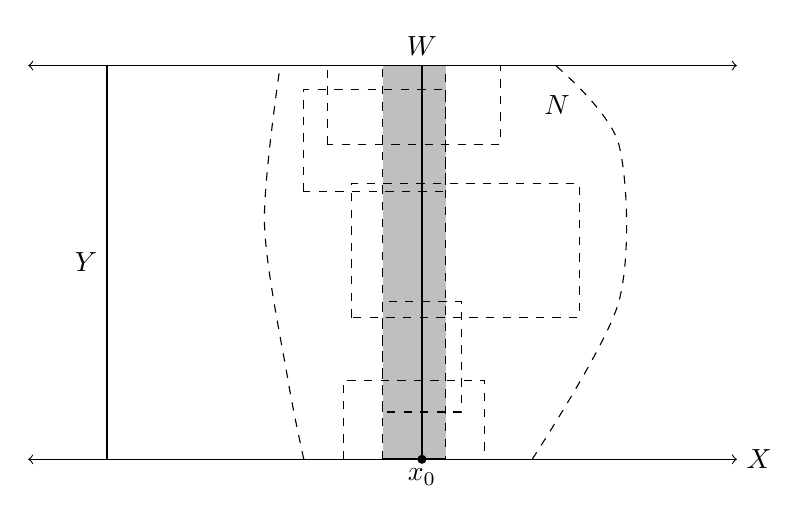
\begin{tikzpicture}
        \draw[dashed, fill=lightgray] (3.5,0) rectangle (4.3,5);
        \draw (0,0)--(0,5);
        \draw[<->] (-1,0)--(8,0);
        \node[right] at (8,0) {$X$};
        \node[left] at (0,2.5) {$Y$};
        \draw[<->] (-1,5)--(8,5);
        \draw[thick] (4,0)--(4,5);
        \draw[dashed] (3,0) rectangle (4.8,1);
        \draw[dashed] (3.5,0.6) rectangle (4.5,2);
        \draw[dashed] (3.1,1.8) rectangle (6,3.5);
        \draw[dashed] (2.5,3.4) rectangle (4.3,4.7);
        \draw[dashed] (2.8,4) rectangle (5, 5);
        \draw[thick] (3.5,0)--(4.3,0);
        \node[above] at (4,5) {$W$};
        \node[below] at (4,0) {$x_0$};
        \draw[fill] (4,0) circle (0.05);
        \draw[dashed] plot [smooth] coordinates {(2.5,0) (2.3, 1) (2,3) (2.2,5)};
        \draw[dashed] plot [smooth] coordinates {(5.4,0) (6.5,2) (6.5,4) (5.7,5)};
        \node[left] at (6,4.5) {$N$};
      \end{tikzpicture}
      \label{fig:tube_lemma}
    \end{figure}
  \end{lemma}
  \begin{proof}
    Let us cover $x_0 \times Y$ by basis elements $U \times V$ (for the topology of $X \times Y$) lying in $N$. The space $x_0$ is compact since it is homeomorphic to $Y \implies$ we can cover $x_0 \times Y$ by finitely such basis elements
    \begin{equation}
      U_1 \times V_1, U_2 \times V_2, \ldots , U_n \times V_n
    \end{equation}
    Without loss of generality, we can assume that each $U_i \times V_i$ has a nontrivial intersection with $x_0 \times Y$, since otherwise, it would be superfluous. Now, we define the intersection of all the open neighborhoods of $x_0$ in $X$ of the basis elements $U_i \times V_i$. That is, let
    \begin{equation}
      W \coloneqq \bigcup_{i=1}^n U_i
    \end{equation}
    As an intersection of open sets, $W$ is also open containing $x_0$. With this well-defined tube $W \times Y$, we claim that it is entirely contained within $N$. That is, given a point $x \times y \in W \times Y$, consider the corresponding point $x_0 \times y$ that is the image of the projection of $x\times y$ onto $x_0 \times Y$. Clearly, $x_0 \times y$ belongs to some $U_k \times V_k$ (for some $k$) $\implies y \in V_k$. Since $x \in W$, $x$ is clearly in $U_k$, meaning that $x \times y \in U_k \times V_k \subset N$, as desired. 
  \end{proof}

  \begin{theorem}[Finite Products]
    The product of finitely many compact spaces is compact. 
  \end{theorem}
  \begin{proof}
    Using induction, it suffices to prove that the product of 2 compact spaces is compact. Let $X$ and $Y$ be compact spaces. By the tube lemma, for each $x \in X$, there exists a neighborhood $W_x$ of $x$ such that the tube $W_x \times Y$ can be covered with finitely (by compactness of $Y$) many open sets in $X \times Y$. The collection of all neighborhoods $W_x$ is an open covering of $X$. By compactness of $X$, there exists a finite subcollection
    \begin{equation}
      W_1, W_2, \ldots , W_k
    \end{equation}
    covering $X$. The finite union of the tubes 
    \begin{equation}
      \bigcup_{i=1}^k W_i \times Y
    \end{equation}
    clearly covers $X \times Y$, meaning that $X \times Y$ is compact. 
  \end{proof}

  \begin{theorem}[Tychonoff Theorem]
    An arbitrary product of compact spaces is compact under the product topology. 
  \end{theorem}
  \begin{proof}
    
  \end{proof}

  \begin{definition}[Finite Intersection Condition]
    A collection $\mathcal{C}$ of subsets of $X$ is said to satisfy the \textbf{finite intersection condition} if for every finite subcollection 
    \begin{equation}
      \{\mathcal{C}_1, \mathcal{C}_2, \ldots , \mathcal{C}_n\}
    \end{equation}
    of $\mathcal{C}$, the intersection
    \begin{equation}
      \bigcap_{i=1}^n \mathcal{C}_i
    \end{equation}
    is nonempty. 
  \end{definition}

  Clearly, the empty sets cannot below to any collection with the finite intersection property. Additionally, the condition is trivially satisfied if the intersection over the entire collection is non-empty or if the collection is nested. However, here is one example that does satisfy the finite intersection condition. 

  \begin{example}
    Let $X = (0,1)$ and for each positive integer $i$, $X_i$ is the set of elements of $X$ having a decimal expansion with digit $0$ in the $i$th decimal place. Then, any finite intersection of $X_i$'s is nonempty, but the intersection of all $X_i$ for $i \in \mathbb{N}$ is empty, since no element of $(0,1)$ has all zero digits. 
  \end{example}

  Here is an analogous example to the previous one. 

  \begin{example}
    In the space $\mathbb{R}$, let us define $C_i \coloneqq \mathbb{R} \setminus \{i\}$. That is, $C_i$ is $\mathbb{R}$ missing a point at $i$. Then, the collection of all $C_i$'s does satisfy the finite intersection condition. We show below the finite intersection of the five subsets $C_0, C_1, C_2, C_3, C_4$. 

    \begin{figure}[H]
      \centering 
      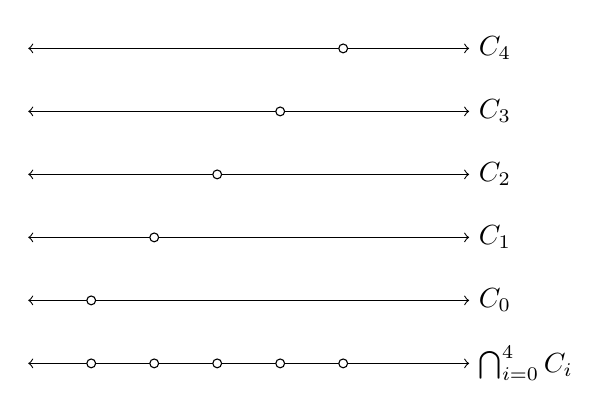
\begin{tikzpicture}[scale=0.8]
        \draw[<->] (-1,0)--(6,0);
        \draw[<->] (-1,1)--(6,1);
        \draw[<->] (-1,2)--(6,2);
        \draw[<->] (-1,3)--(6,3);
        \draw[<->] (-1,4)--(6,4);
        \draw[<->] (-1,-1)--(6,-1);
        \draw[fill=white] (0,0) circle (0.07); 
        \draw[fill=white] (1,1) circle (0.07); 
        \draw[fill=white] (2,2) circle (0.07); 
        \draw[fill=white] (3,3) circle (0.07); 
        \draw[fill=white] (4,4) circle (0.07); 
        \draw[fill=white] (0,-1) circle (0.07); 
        \draw[fill=white] (1,-1) circle (0.07); 
        \draw[fill=white] (2,-1) circle (0.07); 
        \draw[fill=white] (3,-1) circle (0.07); 
        \draw[fill=white] (4,-1) circle (0.07); 
        \node[right] at (6,-1) {$\bigcap_{i=0}^4 C_i$};
        \node[right] at (6,0) {$C_0$};
        \node[right] at (6,1) {$C_1$};
        \node[right] at (6,2) {$C_2$};
        \node[right] at (6,3) {$C_3$};
        \node[right] at (6,4) {$C_4$};
      \end{tikzpicture}
      \label{fig:ex}
    \end{figure}
  \end{example}

  \begin{theorem}
    Let $X$ be a topological space. Then $x$ is compact if and only if for any collection $\mathcal{C}$ of closed sets in $X$ satisfying the finite intersection condition, the intersection 
    \begin{equation}
      \bigcap_{C \in \mathcal{C}} C
    \end{equation}
    of all the elements of $\mathcal{C}$ is nonempty. 
  \end{theorem}
  \begin{proof}
    Given a collection $S$ fo subets of $X$, let 
    \begin{equation}
      \mathcal{C} \coloneqq \{X \setminus A \; | \; A \in S\}
    \end{equation}
    be the collection of their complements. Then, the following statements hold 
    \begin{enumerate}
      \item $S$ is a collection of open sets if and only if $\mathcal{C}$ is a collection of closed sets. 
      \item The collection $S$ covers $X$ if and only if the intersection 
      \begin{equation}
        \bigcap_{C \in \mathcal{C}} C
      \end{equation}
      of all the elements of $\mathcal{C}$ is empty. 

      \item The finite subcollection $\{A_1, A_2, \ldots , A_n\}$ of $S$ covers $X$ if and only if the intersection of the corresponding elements $C_i \coloneqq X \setminus A$ of $\mathcal{C}$ is empty. 
    \end{enumerate}
    Clearly, (1) is trivial, and (2) and (3) follows from DeMorgan's Law. 
    \begin{equation}
      X \setminus \bigcup_{\alpha \in J} A_\alpha = \bigcap_{\alpha \in J} (X \setminus A_\alpha)
    \end{equation}
    Using statement 3, the existence of a finite collection of closed sets $C$ in $X$ satisfying the finite intersection condition is equivalent to its complements (which are open sets) covering $X$, which is precisely the definition of compactness. 
  \end{proof}

  Clearly, the previous example in the real line $\mathbb{R}$ shows that $\mathbb{R}$ is indeed not compact. 

  \begin{corollary}
    The space $X$ is compact if and only if every collection $\C$ of subsets of $X$ satisfying the finite intersection condition, the intersection 
    \begin{equation}
      \bigcap_{A \in \C} \bar{A}
    \end{equation}
    of their closures is nonempty. 
  \end{corollary}

\subsection{Limit Point Compactness}

  We now state different, weaker types of compactness. 

  \begin{definition}[Limit Point Compactness]
    A space $X$ is said to be \textbf{limit point compact} if every infinite subset of $X$ has a limit point. 
  \end{definition}

  \begin{theorem}
    Compactness $\implies$ limit point compactness.  
  \end{theorem}

  \begin{lemma}[Lebesgue Number Lemma]
    Let $\C$ be an open covering of the metric space $(X, d)$. If $X$ is compact, then there is a $\delta > 0$ such that for each subset of $X$ having diameter than $\delta$, there exists an element of $\C$ containing it. This number $\delta$ is called a \textbf{Lebesgue number} for the covering $\C$. 
  \end{lemma}

\subsection{Preservation of Limit Point Compactness}

\subsection{Sequential Compactness}

  \begin{definition}[Sequentially Compact]
    A space $X$ is said to be \textbf{sequentially compact} if every sequence of points in $X$ has a subsequence that converges to a point $x \in X$. 
  \end{definition}

  \begin{theorem}[Equivalence of Compactness in Metrizable Spaces]
    Let $(X, \T)$ be a metrizable space. Then the following are equivalent: 
    \begin{enumerate}
      \item $X$ is compact. 
      \item $X$ is limit point compact. 
      \item $X$ is sequentially compact. 
      \item $X$ is countably compact. 
    \end{enumerate}
  \end{theorem}

\subsection{Preservation of Sequential Compactness}

\subsection{Local Compactness}

  \begin{definition}[Locally Compact]
    A space $X$ is said to be \textbf{locally compact} at $x$ if there is some compact subset $C$ of $X$ that contains a neighborhood of $x$. If $X$ is locally compact at each of its points, $X$ is simply to be \textbf{locally compact}. 
  \end{definition}

  \begin{example}
    The real line $\mathbb{R}$ is locally compact since any point $x \in \mathbb{R}$ lies within a certain closed interval $[a,b]$, which is compact. The subspace $\mathbb{Q}$ is not locally compact. 
  \end{example}

  Two of the most well-behaved classes of spcaes to deal with are metrizable spaces and compact Hausdorff spaces. If a given space is not one of these types, the next best thing one can hope for is that it is a subspace of one of these spaces. Clearly, a subspace of a metrizable space is itself metrizable, so one does not get any new spaces this way. However, a subspace of a compact Hausdorff space need not be compact. This leads to the question: Under what conditions is a space homeomorphic to a subspace of a compact Hausdorff space? 

  \begin{definition}[Compactification]
    Let $X$ be a locally compact Hausdorff space. Take some object outside $X$, denoted by the symbol $\infty$, and adjoin it to $X$, forming the set
    \begin{equation}
      Y = X \cup \{\infty\}
    \end{equation}
    Topologize $Y$ by defining the collection of open sets in $Y$ to be the sets of the following types:
    \begin{enumerate}
      \item $U$, where $U$ is an open subset of $X$. 
      \item $Y \setminus C$, where $C$ is a compact subset of $X$.
    \end{enumerate}
    Then, this space $Y$ is called the \textbf{one-point compactification of $X$}. This is in some sense the minimal compactification of $X$. 
  \end{definition}

  We briefly show that this set of open sets on $Y$ is indeed a topology. First, $\emptyset$ is of type 1 and $Y$ itself is of type 2. Given $U_i$ of type 1 and $Y \setminus C_i$ of type 2, we have the intersections of two sets
  \begin{align*}
    &U_1 \cap U_2 & \text{ is type 1} \\
    &(Y \setminus C_1) \cap (Y \setminus C_2) = Y \setminus (C_1 \cup C_2) & \text{ is type 2} \\
    &U_1 \cap (Y \setminus C_1) = U_1 \cap (X \setminus C_1) & \text{ is type 1} 
  \end{align*}
  along with the arbitrary union of sets
  \begin{align*}
    &\bigcup U_\alpha = U & \text{ is type 1} \\
    &\bigcup (Y \setminus C_\beta) = Y \setminus (\bigcap C_\beta) = Y \setminus C & \text{ is type 2} \\
    &(\bigcup U_\alpha) \cup ( \bigcup (Y \setminus C_\beta)) = U \cup (Y \setminus C) = Y \setminus (C \setminus U) & \text{ is type 2}
  \end{align*}
  We now present some properties of one-point compactifications. 

  \begin{theorem}
    Let $X$ be a locally compact Hausdorff space which is not compact, and let $Y$ be a one-point compactification of $X$. Then $Y$ is a compact Hausdorff space. Additionally, since $X \subset Y$ with $Y \setminus X$ consisting of a single point, $\bar{X} = Y$. 
  \end{theorem}

  \begin{example}[Extended Real Number Line]
    The one-point compactification of the real line $\mathbb{R}$ is homeomorphic to the circle $S^1$. That is, 
    \begin{equation}
      \mathbb{R} \cup \{\infty\} \cong S^1
    \end{equation}
    $\mathbb{R} \cup \{\infty\}$ is called the \textbf{extended real number line}. 
    
    \begin{figure}[H]
      \centering 
      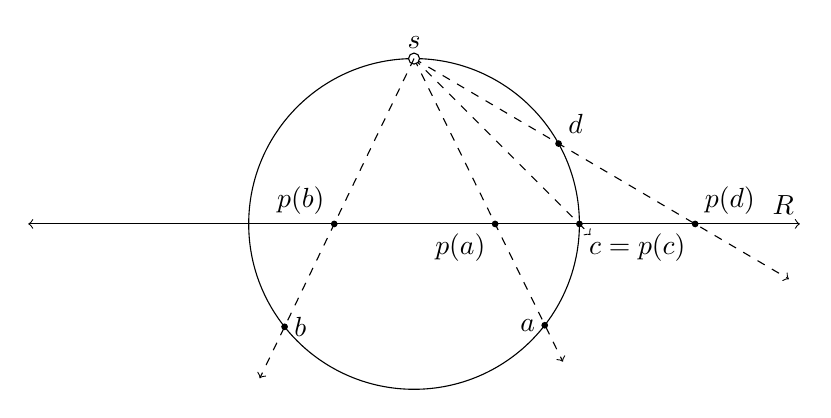
\begin{tikzpicture}[scale=0.7]
        \draw (0,0) circle (3);
        \node[above] at (0,3) {$s$};
        \draw[<->] (-7,0)--(7,0);
        \node[above] at (6.7,0) {$\mathbb{R}$};
        \draw[->, dashed] (0,3)--(3.2,-0.2);
        \draw[->, dashed] (0,3)--(2.7,-2.5);
        \draw[->, dashed] (0,3)--(6.8,-1);
        \draw[fill=white] (0,3) circle (0.1);
        \draw[->, dashed] (0,3)--(-2.8, -2.8);
        \draw[fill] (3,0) circle (0.05);
        \draw[fill] (-2.349,-1.866) circle (0.05);
        \draw[fill] (5.1,0) circle (0.05);
        \draw[fill] (2.622,1.458) circle (0.05);
        \draw[fill] (-1.448,0) circle (0.05);
        \draw[fill] (1.471,0) circle (0.05); 
        \draw[fill] (2.371, -1.838) circle (0.05);
        \node[left] at (2.371, -1.838) {$a$};
        \node[below left] at (1.471,0) {$p(a)$};
        \node[above left] at (-1.448,0) {$p(b)$};
        \node[right] at (-2.349,-1.866) {$b$};
        \node[above right] at (5.1,0) {$p(d)$};
        \node[above right] at (2.622,1.458) {$d$};
        \node[below right] at (3,0) {$c = p(c)$};
      \end{tikzpicture}
      \caption{We can visualize this homeomorphism by visualizing the stereographic projection $p: S^1 \setminus \{s\} \rightarrow \mathbb{R}$. } 
      \label{fig:extended_r}
    \end{figure}
  \end{example}

  \begin{example}[2-Sphere]
    The one point-compactification of the real plane $\mathbb{R}^2$ is homeomorphic to the 2-sphere $S^2$. That is, 
    \begin{equation}
      \mathbb{R}^2 \cup \{\infty\} \cong S^2
    \end{equation}
  \end{example}

  \begin{lemma}
    Let $X$ be a Hausdorff space. Then $X$ is locally compact at $x$ if and only if for every neighborhood $U$ of $x$, there is a neighborhood $V$ of $x$ such that $\bar{V}$ is compact and $\bar{V} \subset U$. 
  \end{lemma}

  \begin{corollary}
    Let $X$ be a locally compact Hausdorff space with $Y$ a subspace of $X$. If $Y$ is closed in $X$ or open in $X$, then $Y$ is locally compact. 
  \end{corollary}

  \begin{corollary}
    A space $X$ is homeomorphic to an open subset of a compact Hausdorff space if and only if $X$ is locally compact and Hausdorff. 
  \end{corollary}

\subsection{Countable Compactness}

  \begin{definition}[Countably Compact]
    A space $X$ is said to be \textbf{countably compact} if every countably open cover has a finite subcover. 
  \end{definition}

\subsection{Lindelof Spaces} 

  \begin{definition}[Lindelof Space]
    A space for which every open covering contains a countable subcovering is called a \textbf{Lindelof space}. 
  \end{definition}

\subsection{Compactifications}
  
  \begin{definition}
    A \textbf{compactification} of a space $X$ is a compact Hausdorff space $Y$ containing $X$ such that $X$ is dense in $Y$ (that is $\bar{X} = Y$). Two compactifications $Y_1$ and $Y_2$ of $X$ are said to be \textbf{equivalent} if there is a homeomorphism $h: Y_1 \longrightarrow Y_2$ such that $h(x) = x$ for every $x \in X$. 
  \end{definition}

  \begin{theorem}
    Let $X$ be completely regular, and let $\beta(X)$ be its Stone-Cech compatification. Then every bounded continuous real-valued function on $X$ can be uniquely extended to a continuous real-valued function on $\beta(X)$. 
  \end{theorem}

  \begin{lemma}
    Let $A \subset X$, and let $f: A \longrightarrow Z$ be a continuous map of $A$ into the Hausdorff space $Z$. There is at most one extension of $f$ to a continuous function $g: \bar{A} \longrightarrow Z$. 
  \end{lemma}

  \begin{theorem}
    Let $X$ be completely regular. Let $Y_1, Y_2$ be two compactifications of $X$ having the extension property. Then there is a homeomorphism $\phi$ of $Y_1$ onto $Y_2$ such that $\phi(x) = x$ for each $x \in X$. 
  \end{theorem}

\subsection{Exercises}

  \begin{exercise}[Munkres 27.2]
    Let $X$ be a metric space with metric $d$; let $A \subset X$ be nonempty.
    \begin{enumerate}
      \item[(a)] Show that $d(x, A) = 0$ if and only if $x \in \overline{A}$.
      \item[(b)] Show that if $A$ is compact, $d(x, A) = d(x, a)$ for some $a \in A$.
      \item[(c)] Define the $\epsilon$-neighborhood of $A$ in $X$ to be the set
        \[
          U(A, \epsilon) = \{x \mid d(x, A) < \epsilon\}.
        \]
        Show that $U(A, \epsilon)$ equals the union of the open balls $B_d(a, \epsilon)$ for $a \in A$.
      \item[(d)] Assume that $A$ is compact; let $U$ be an open set containing $A$. Show that some $\epsilon$-neighborhood of $A$ is contained in $U$.
      \item[(e)] Show the result in (d) need not hold if $A$ is closed but not compact.
    \end{enumerate}
  \end{exercise}
  \begin{solution}
    For (a), we prove bidirectionally. 
    \begin{enumerate}
      \item $(\rightarrow)$. We prove the contrapositive. Let $x \not\in \overline{A} \implies \exists$ $B(x, \epsilon)$ satisfying $B(x, \epsilon) \cap A \neq \emptyset$. This means that $d(x, A) \geq \epsilon > 0$. Note that $x \not\in A$ means that the actual point $x$ can't intersect $A$, while $x \not\in A^\prime$ means that the punctured ball can't intersect $A$. If $x \not\in A^\prime$, then $d(x, A) = 0$ if $x$ is an isolated point. 

      \item $(\leftarrow)$. If $x \in \overline{A}$, then for every $\epsilon > 0$, $B(x, \epsilon) \cap A \neq 0$. Therefore, $0 \leq d(x, A) < \epsilon$ for all positive $\epsilon$, which implies that $d(x, A) = 0$. 
    \end{enumerate}
    For (b). Since the metric $d$ is continuous, the function $f(y) = d(x, y)$ is continuous over compact $A$, and by EVT, $f$ achieves its minimum in $A$. Call this point $a \in A$, and so we have $d(x, a) \leq d(x, A)$. However, $d(x, A) \leq d(x, a)$ for all $a \in A$ by definition, so $d(x, a) = d(x, A)$. 

    For (c), we prove bidirectionally. 
    \begin{enumerate}
      \item $U(A, \epsilon) \subset \cup_{a \in A} B(a, \epsilon)$. Let $x \in U(A, \epsilon)$, and so we have $d(x, A) < \epsilon$. We see that $d(x, A) = \inf \{d(x, a) \mid a \in A\}$, so $\epsilon > d(x, A)$ cannot be a lower bound. Therefore by definition there exists some $a^\ast \in A$ satisfying $d(x, a^\ast) < \epsilon \implies x \in B(a^\ast, \epsilon)$. 

      \item $\cup_{a \in A} B(a, \epsilon) \subset U(A, \epsilon)$. Let $x \in \cup_{a \in A} B(a, \epsilon)$. Then we pick a particular $a^\ast$ such that $x \in B(a^\ast, \epsilon)$, which satisfies $d(x, a^\ast) < \epsilon$. Since $a^\ast \in A$, $d(x, A) \leq d(x, a^\ast) < \epsilon \implies x \in U(A, \epsilon)$
    \end{enumerate}

    For (d), we first construct the open cover $\mathscr{B} = \{B(a, \epsilon(a))\}_{a \in A}$ consisting of all neighborhoods of $a$ with some $\epsilon = \epsilon(a)$ (that may be dependent on $a$) such that $B(a, 2\epsilon(a)) \subset U$. This is possible since $U$ is open. $\mathscr{B}$ is an open cover of compact $A$, so take a finite subcover $\mathscr{F} = \{B(a_i, \epsilon(a_i))\}_{i=1}^n$ with the minimum $\epsilon = \min_i \{\epsilon_i\}$. We claim that 
    \begin{equation}
      A \subset \bigcup_i B(a_i, \epsilon) \subset U(A, \epsilon) \subset \bigcup_i B(a_i, 2\epsilon) \subset U
    \end{equation} 
    The first inclusion is trivial since $\mathscr{F}$ is an open cover. The second follows directly from (c) since $U(A, \epsilon)$ contains the union of all open balls of the form $B(a, \epsilon)$, which contains those with center $a_i$. The fourth subset is by construction. As for the third subset, we claim that if $x \in U(A, \epsilon)$, then by (b) there exists some $y \in A$ s.t. $d(x, y) < \epsilon$. Also, since $y \in A \subset \cup_i B(a_i, \epsilon)$, we have $d(y, a_i) < \epsilon$ for some $a_i$. Therefore, by the triangle inequality, 
    \begin{equation}
      d(x, a_i) <  d(x, y) + d(y, a_i) = \epsilon + \epsilon = 2\epsilon  
    \end{equation}
    and so $x \in B(a_i, 2\epsilon)$ for some $a_i$, and so $x \in \cup_i B(a_i, 2\epsilon) \subset U$. 

    For (e), consider the y-axis $\{0\} \times \mathbb{R}$ (a product of closed sets) and the open set from Munkres's Tube Lemma example
    \begin{equation}
      U = \{(x, y) \in \mathbb{R}^2 \mid |x| < 1/(y^2 + 1)\}
    \end{equation}
    $U$ is open, but given any $\epsilon > 0$, $U(A, \epsilon) = (-\epsilon, +\epsilon) \times \mathbb{R}$ is not contained in $U$ since by the Archimidean property, we can set $y$ arbitrarily large so that 
    \begin{equation}
      \frac{1}{y^2 + 1} < \epsilon
    \end{equation} 
    and letting $\delta$ be a number between them, we have $(\delta, y) \in U(A, \epsilon)$ but not in $U$ since $1/(y^2 + 1) < \delta$. 
  \end{solution}

  \begin{exercise}[Munkres 27.6]
    Let $A_0$ be the closed interval $[0, 1]$ in $\mathbb{R}$. Let $A_1$ be the set obtained from $A_0$ by deleting its ``middle third'' $(\frac{1}{3}, \frac{2}{3})$. Let $A_2$ be the set obtained from $A_1$ by deleting its ``middle thirds'' $(\frac{1}{9}, \frac{2}{9})$ and $(\frac{7}{9}, \frac{8}{9})$. In general, define $A_n$ by the equation
    \[
      A_n = A_{n-1} - \bigcup_{k=0}^{\infty}\left(\frac{1+3k}{3^n}, \frac{2+3k}{3^n}\right).
    \]
    
    The intersection
    \[
      C = \bigcap_{n\in\mathbb{Z}_+} A_n
    \]
    is called the Cantor set; it is a subspace of $[0, 1]$.
    \begin{enumerate}
      \item[(a)] Show that $C$ is totally disconnected.
      \item[(b)] Show that $C$ is compact.
      \item[(c)] Show that each set $A_n$ is a union of finitely many disjoint closed intervals of length $1/3^n$; and show that the end points of these intervals lie in $C$.
      \item[(d)] Show that $C$ has no isolated points.
      \item[(e)] Conclude that $C$ is uncountable.
    \end{enumerate}
  \end{exercise}
  \begin{solution}
    \begin{enumerate}
      \item For (a), pick distinct $x, y \in C$ and WLOG let $x < y$. Then $y - x > 0$, and so by the Archimidean property we can find some $n$ s.t. 
      \begin{equation}
        y - x > \frac{1}{3^{n-2}} 
      \end{equation} 
      Furthermore, we can multiply both sides of the left equation by $3^n$ to get 
      \begin{equation}
        3^n y - 3^n x > 9
      \end{equation}
      which implies that there exists a natural $a \in \mathbb{N}$ s.t. 
      \begin{equation}
        3^n x < a < a + 1 < \ldots < a + 8 < 3^n y 
      \end{equation}
      There must be a divisor amongst the $a, a + 1, a + 2$, so call it $a^\prime = 3k$. Then we must have 
      \begin{equation}
        3^n x < 3k < 3k + 1 < 3k + 2 < 3^n y \implies x < \frac{3k}{3^n} < \frac{1 + 3k}{3^n} < \frac{2 + 3k}{3^n} < y
      \end{equation} 
      and so we know that the middle interval $(\frac{1 + 3k}{3^n}, \frac{2 + 3k}{3^n})$ is not included in $C$. Pick any point $y \in (\frac{1 + 3k}{3^n}, \frac{2 + 3k}{3^n})$ and so $[0, y) \cap C$ and $(y, 0] \cap C$ is a separation. Since $x, y$ were arbitrary, $C$ is totally disconnected. 

      \item For (b), $C$ is bounded, so it suffices to show that it is closed. We claim that $A_n$ is closed for all $n \in \mathbb{N}$. This is because $A_0$ is closed. Now given that $A_{n-1}$ is closed, the intervals that are taken out are each open since they are open intervals, and their arbitrary union is also open. Therefore, let's call this $U_{n-1}$, and so 
      \begin{equation}
        A_{n-1} \setminus \bigcup_{k=0}^\infty \bigg( \frac{1 + 3k}{3^n}, \frac{2 + 3k}{3^n} \bigg) = A_{n-1} \setminus U_{n-1} = A_{n-1} \cap (U_{n-1})^c 
      \end{equation} 
      where the complement (in $[0, 1]$) is closed and so the intersection of closed sets is closed. Finally, $C$ which is the intersection of closed sets $A_n$ is closed. 

      \item We prove using induction. Clearly $A^0 = [0, 1]$ has a length of $ 1/3^0 = 1$ with endpoints $0, 1$, and $A_1 = [0, 1/3] \cup [2/3, 1]$ consists of two intervals of length $1/3^1$ with endpoints $\{0, 1/3, 2/3, 1\}$ which contains the endpoints of $A_0$ and cover all multiples of $1/3^1$. Now given that $A_n$ is a finite disjoint union of intervals of length $1/3^n$ of the form 
      \begin{equation}
        I = \bigg[ \frac{a}{3^n}, \frac{a+1}{3^n} \bigg] = \bigg[ \frac{3a}{3^{n+1}}, \frac{3a + 3}{3^{n+1}} \bigg]
      \end{equation}
      with endpoints that have a 1-to-1 correspondence with all multiples of $1/3^n$, we label the left and right endpoints as $l = l_I, u = u_I$ for convenience. Now for $A_{n+1}$ we claim that for each $I$, 
      \begin{equation}
        I \cap \bigg( \bigcup_{k=0}^\infty \Big( \frac{1 + 3k}{3^{n+1}}, \frac{2 + 3k}{3^{n+1}} \Big) \bigg) = \bigg( \frac{1 + 3a}{3^{n+1}}, \frac{2 + 3a}{3^{n+1}} \bigg)
      \end{equation}
      because 
      \begin{equation}
        \ldots < 3a - 1 = 2 + 3(a - 1) < 3a < 1 + 3a < 2 + 3a < 3a + 3 < 1 + 3(a + 1) = 3a + 4 < \ldots
      \end{equation} 
      and so every interval $I$ would be divided into two disjoint intervals 
      \begin{equation}
        I = \bigg[ \frac{3a}{3^{n+1}}, \frac{1 + 3a}{3^{n+1}} \bigg] \sqcup \bigg[ \frac{2 + 3a}{3^{n+1}}, \frac{3 + 3a}{3^{n+1}} \bigg] = I_1 \sqcup I_2
      \end{equation}
      each of length $1/3^{n+1}$ and endpoints changed from 
      \begin{equation}
        \bigg\{ \frac{3a}{3^{n+1}}, \frac{3 + 3a}{3^{n+1}} \bigg\} \mapsto \bigg\{ \frac{3a}{3^{n+1}}, \frac{1 + 3a}{3^{n+1}}, \frac{2 + 3a}{3^{n+1}}, \frac{3 + 3a}{3^{n+1}} \bigg\} 
      \end{equation}
      which are also consecutive multiples of $1/3^{n+1}$ that will cover all multiples of $1/3^{n+1}$ when taking all intervals $I$.  Therefore, the number of intervals will double, which is still finite. The two subintervals also still disjoint from each other since $1 + 3a < 2 + 3a$, and they are disjoint from all other intervals since their extensions (before the middle interval was taken out) was disjoint. Finally, $l$ is the left endpoint of $I_1$ and $u$ is the right endpoint of $I_2$, and so an endpoint of any $A_n$ is an endpoint of $A_m$ for $m \geq n$, which implies that every endpoint lies in $C$. 
      
      \item Given $x \in C$, let us take the $\epsilon$-neighborhood $(x - \epsilon, x + \epsilon)$. Then by Archimidean property, we can choose a large $n \in \mathbb{N}$ s.t. $\frac{1}{3^{n-2}} < \epsilon$, and so 
      \begin{equation}
        9 < 3^{n} \epsilon \implies 9 < 3^n (x + \epsilon) - 3^n x
      \end{equation}
      and so there are naturals $a, a+1, \ldots, a+8$ in between $3^n x$ and $3^n (x + \epsilon)$. One of $a, a+1, a+2$ must be a multiple of three, and call it $a^\ast = 3k$. Then 
      \begin{equation}
        3^n x < 1 + 3k < 2 + 3k < 3^n (x + \epsilon) \implies x < \frac{1 + 3k}{3^n} < \frac{2 + 3k}{3^n} < 3^n (x + \epsilon)
      \end{equation}
      But $(1 + 3k)/3^n$ is an endpoint of an interval in $A_n$, particularly $\big[\frac{1+3k}{3^n}, \frac{2 + 3k}{3^n} \big]$, which is guaranteed to exist since we've proved that the endpoints of the disjoint intervals cover all multiples of $1/3^n$ and also are in $C$.  

      \item We have proved that $C$ is compact and has no isolated points. $C$ as a subset of Hausdorff $[0, 1]$ is also Hausdorff. So as a compact Hausdorff space with no isolated points it is uncountable. 
    \end{enumerate}
  \end{solution}

  \begin{exercise}[Munkres 28.2]
    Show that $[0, 1]$ is not limit point compact as a subspace of $\mathbb{R}_\ell$. 
  \end{exercise}
  \begin{solution}
    Consider the set $A = \{a_n\} = \{1 - \frac{1}{n} \}_{n \in \mathbb{N}}$. $a \in A$ is not a limit point since we can see that if $a = 1 - \frac{1}{k}$, we can see that setting $\epsilon = \frac{1}{2k (k+1)}$ gives 
    \begin{equation}
      a + \epsilon = 1 - \frac{2(k+1)}{2k(k+1)} + \frac{1}{2k (k+1)} = 1 - \frac{2k + 1}{2k(k+1)} < 1 - \frac{2k}{2k(k+1)} < 1 - \frac{1}{k+1} 
    \end{equation}
    and the opposite side with $a - \epsilon$ also holds since $d(a_{k-1}, a_k) > d(a_k, a_{k+1})$. 
    \begin{equation}
      \bigg(1 - \frac{1}{k-1} \bigg) - \bigg(1 - \frac{1}{k} \bigg) = \frac{1}{k(k-1)} > \frac{1}{k(k+1)} = \bigg(1 - \frac{1}{k} \bigg) - \bigg(1 - \frac{1}{k+1} \bigg) 
    \end{equation}
    and so $[a - \epsilon, a + \epsilon)$ does not intersect $A$. Now pick $x \in (0, 1) \setminus A$. Then there exists unique natural $n \in \mathbb{N}$ such that 
    \begin{equation}
      n < \frac{1}{x} < n + 1 \implies \frac{1}{n+1} < x < \frac{1}{n}
    \end{equation}
    and so we can set $\epsilon = \min\{\frac{1}{n}, \frac{1}{n+1}\}$ to create an open ball around $x$ not intersecting $A$. Now $0$ is not a limit point since we can choose $\epsilon = 1/3$, and so $B(0, 1/3) \cap [0, 1] = [0, 1/3)$ does not intersect $A$ which has all elements at least $1/2$. Finally $1$ is not a limit point since we can choose the singleton set $\{1\} = [1, 2) \cap [0, 1]$ that does not intersect $A$. Therefore $[0, 1]$ has an infinite subset that does not have a limit point, so it is not limit point compact. 
  \end{solution}


